\subsection{Inhoudstypen}\label{inhoudstypen}
Inhoudstypen worden gebruikt voor het weergeven van verschillende typen inhoud. Per inhoudstype kunnen bijvoorbeeld verschillende velden gedefinieerd worden en de bijbehorende pagina's kunnen apart gestijled worden. Het gebruik van inhoudstypen cre�ert veel flexibiliteit.

In de volgende paragraaf zullen specifieke inhoudstypen nader beschreven worden.

\subsubsection{Agenda}\label{agenda}

\begin{enumerate}
\item Vul een titel in bij het veld 'Titel'
\item Vul optioneel een introductie tekst in bij het veld 'Intro'
\item Vul de hoofdtekst in bij het veld 'Body'
\item Upload optioneel een afbeelding bij het veld 'Image'
\item Specificeer optioneel een (eind)datum - kruis 'toon einddatum' aan om een einddatum te specificeren
\item Specificeer optioneel een datum en tijd (bijvoorbeeld wanneer een evenement start) bij het veld 'Datum'
\item Specificeer optioneel een locatie (van bijvoorbeeld een evenement) bij het veld 'Locatie'
\item Voeg optioneel de content toe aan de kalender, dit doe je d.m.v. een datum te specificeren bij het veld 'Datum'
\item Klik onderaan de pagina op de knop 'Opslaan' om de inhoud op te slaan.
\end{enumerate}

\subsubsection{Bekendmaking}\label{bekendmaking}

\begin{enumerate}
\item Vul een titel in bij het veld 'Titel'
\item Selecteer het type bekendmaking
\item Voeg optioneel de content toe aan de kalender, dit doe je d.m.v. een datum te specificeren bij het veld 'Datum'
\item Vul de hoofdtekst in bij het veld 'Body'
\item Specificeer optioneel een locatie (van bijvoorbeeld een evenement) bij het veld 'Locatie'
\item Klik onderaan de pagina op de knop 'Opslaan' om de inhoud op te slaan.
\end{enumerate}

\subsubsection{Bericht}\label{bericht}

\begin{enumerate}
\item Vul een titel in bij het veld 'Titel'
\item Vul de hoofdtekst in bij het veld 'Body'
\item Klik onderaan de pagina op de knop 'Opslaan' om de inhoud op te slaan.
\end{enumerate}

\subsubsection{Bestand}\label{bestand}

\begin{enumerate}
\item Vul een titel in bij het veld 'Titel'
\item Upload het gewenste bestand bij het veld 'Bestand'
\item Klik onderaan de pagina op de knop 'Opslaan' om de inhoud op te slaan.
\end{enumerate}

\subsubsection{Bestemmingsplan}\label{bestemmingsplan}
Bestemmingsplan

\subsubsection{Blog}\label{blog}
Blog

\subsubsection{Editorial}\label{editorial}
Editorial

\subsubsection{Eenvoudige pagina}\label{eenvoudigepagina}
Eenvoudige pagina

\subsubsection{FAQ}\label{faq}
FAQ

\subsubsection{Forumonderwerp}\label{forumonderwerp}
Forumonderwerp

\subsubsection{Foto}\label{foto}
Foto

\subsubsection{Marktplaats}\label{marktplaats}
Marktplaats

\subsubsection{Nieuws}\label{nieuws}
Nieuws

\subsubsection{Onderwerp}\label{onderwerp}
Onderwerp

\subsubsection{Peiling}\label{peiling}
Peiling

\subsubsection{Persoon}\label{persoon}
Persoon

\subsubsection{Product}\label{product}
Product

\subsubsection{RSS}\label{rss}
RSS

\subsubsection{RSS Source}\label{rsssource}
RSS Source

\subsubsection{Regeling}\label{regeling}
Regeling

\subsubsection{Slide}\label{slide}
Slide

\subsubsection{VAC}\label{vac}
Vac

\subsubsection{Wiki}\label{wiki}
Het inhoudstype 'wiki' zal worden gebruikt voor het aanmaken van informatieve pagina's.

Om een wiki pagina aan te maken ga je naar: \emph{Inhoud toevoegen} $\rightarrow$ \emph{Wiki} , of ga direct naar \drupalpath{node/add/wiki}.

Vul een titel bij het veld 'Titel' en vul informatieve tekst in bij het veld 'Body'.

Voor het inhoudstype 'Wiki' is een speciale filter gebouwd, deze filter maakt het refereren naar andere wiki pagina's mogelijk. 

Het refereren naar een andere wiki pagina gaat als volgt: 

\begin{enumerate}
\item Kopieer de titel van de node waarnaar je wilt refereren, bijvoorbeeld 'wiki pagina'
\item In de body tekst van je huidige node kun je refereren naar de node 'wiki pagina'
\item Plaats de node waarnaar je wilt refereren tussen dubbele 'square brackets': [[wiki pagina]]
\item Bijvoorbeeld: dit is informatie, op de pagina [[wiki pagina]] kun je meer informatie vinden.
\end{enumerate}

\bigskip

\begin{center}
	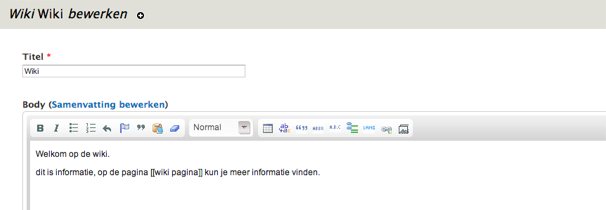
\includegraphics[width=\textwidth]{img/wiki.png}
\end{center}